\usetikzlibrary{patterns}
\usetikzlibrary{arrows}

    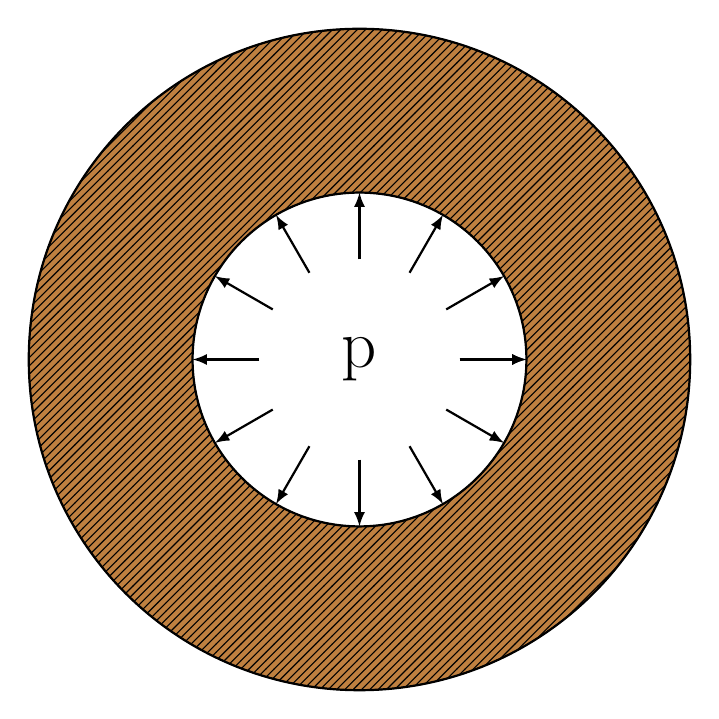
\begin{tikzpicture}
        % draw the coordinates
        %\draw[->] (-1.5cm,0cm) -- (1.5cm,0cm) node[right,fill=white] {$x$};
        %\draw[->] (0cm,-1.5cm) -- (0cm,1.5cm) node[above,fill=white] {$y$};

        % draw the coordinates
        %\draw[->] (-1.5cm,0cm) -- (1.5cm,0cm) node[right,fill=white] {$x$};
        %\draw[->] (0cm,-1.5cm) -- (0cm,1.5cm) node[above,fill=white] {$y$};



	\def \k {2/100 * 0.5}
	\def \R {420}
	\def \r {212}

        % draw the unit circle
        \draw[thick,fill=brown,even odd rule] (0cm,0cm) circle(\R*\k)
        										(0,0) circle(\r*\k);
        						
        						
	\draw[even odd rule,  pattern = north east lines] (0cm,0cm) circle(\R*\k)
        												(0,0) circle(\r*\k);

        \foreach \x in {0,30,...,360} {
                % lines from center to point
                \draw[-latex,thick] (\x:{0.6*\r*\k}) -- (\x:{\r*\k});
                
                %\draw[-latex,thick] (\x:3.75) -- (\x:3);
                % dots at each point
               % \filldraw[black] (\x:1cm) circle(0.4pt);
                % draw each angle in degrees
                %\draw (\x:0.6cm) node[fill=white] {$\x^\circ$};
        }
        
	\node at (0,0) {\Huge p};
        
        
	%\node at (0,6.5) {\large Wheel Scheme};
        
    \end{tikzpicture}